\documentclass[
	aspectratio=169, % default is 43
	8pt, % font size, default is 11pt
	handout, % handout mode without animations, comment out to add animations
]{beamer}

\documentclass[
	aspectratio=169, % default is 43
	8pt, % font size, default is 11pt
	handout, % handout mode without animations, comment out to add animations
]{beamer}

\usepackage{../template/beamerthemeuulm} % use the inofficial uulm beamer theme
\setfaculty{infIngPsy} % set the color scheme for your faculty here [med/infIngPsy/math/nat]

% requires symbolic links
% git clone git@github.com:SoftVarE-Group/SlideTemplate.git C:\Users\...\SlideTemplate
% mklink /J template C:\Users\...\SlideTemplate
% git clone git@spgit.informatik.uni-ulm.de:thuem/slides.git C:\Users\...\ThomasSlides
% mklink /J thomasslides C:\Users\...\ThomasSlides
\graphicspath{{../template/pics/logos}{../template/pics/nature}{../template/pics/uulm}{../thomasslides/}{../pics/people/}{../pics/xkcd/}}

%\usepackage[ngerman]{babel} % use this line for slides in German
%\recordingtrue % special recording mode for use with a greenscreen, gives you space to show yourself in a layer in front of the slides, has no effect in the handout mode

\title{Software Product Lines} % short title is used for the slide footer but optional

% LINKED LITERATURE

\newcommand{\ludewiglichter}{\href{https://learning.oreilly.com/library/view/-/9781457184932/?ar}{Ludewig and Lichter}}
\newcommand{\seeconomics}{\href{https://rds-ulm.ibs-bw.de/link?kid=027381854}{SE Economics}}
\newcommand{\sommervillelink}[1]{\href{https://ulm.ibs-bw.de/aDISWeb/app?service=direct/0/Home/$DirectLink\&sp=SOPAC00\&sp=SAKSWB-IdNr1615420983}{#1}}
\newcommand{\sommerville}{\sommervillelink{Sommerville}}
\newcommand{\thehumbleprogrammer}{\href{https://dl.acm.org/doi/10.1145/1283920.1283927}{The Humble Programmer}}
\newcommand{\thepragmaticprogrammer}{\href{https://learning.oreilly.com/library/view/the-pragmatic-programmer/9780135956977/}{The Pragmatic Programmer}}

% TYPICAL COMMANDS FOR LECTURES

\renewcommand{\emph}[1]{{\color{blue}\textbf{#1}}}

\newcommand{\deutsch}[1]{{\color{blue}(#1)}}
\newcommand{\deutschertitel}[1]{{\tiny\deutsch{#1}}}

\newcommand{\mycite}[1]{``#1''}
\newcommand{\mytitlesource}[1]{{\tiny\normalfont\mbox{[#1]}}}
\newcommand{\mysource}[1]{\ifthenelse{\equal{#1}{}}{}{\phantom{.}~\hfill~\mytitlesource{#1}}}

\newcommand{\todo}[1]{{\color{red}\textbf{[#1]}}}
\newcommand{\fodo}[1]{\todo{\footnote{\todo{#1}}}}
\newcommand{\todots}{\todo{\ldots}}

% IMPORTED PACKAGES

%\usepackage{adjustbox} % used for partofpage
%\usepackage{tcolorbox} % used for mydefinition, mynote, myexample
\usepackage{multicol} % used temporarily for the lecture overview
\usepackage{mathtools} % required for absolute value in modeling lecture

% COMMANDS TO LAYOUT AND ANNIMATE SLIDES

\newcommand{\lessonslearned}[3]{
	\subsection{Summary}
	\begin{frame}{\insertsection -- \insertsubsection}
		\leftorright{
			\mydefinition{Lessons Learned}{
				\begin{itemize}
					#1
				\end{itemize}
			}
			\mynote{Further Reading}{
				\small % references take space, can be a little smaller
				\begin{itemize}
					#2
				\end{itemize}
			}
		}{
			\myexample{Practice}{
				#3
			}
		}
	\end{frame}
}

% TODO temporary hack to layout the slide overview in two colums
\renewcommand{\lectureoverview}{
%	\section*{Overview}
%	\subsection*{Overview}
	\begin{frame}{\insertsubtitle}
		\begin{multicols}{2}
			\tableofcontents
		\end{multicols}
	\end{frame}
}

\renewcommandx{\maketitle}[2][1=apr21-o25a,2=150]{
    {
	\usebackgroundtemplate{} % TODO temporary hack to enable missing pictures at title slide
	%\ifx {#1} \empty \else {\usebackgroundtemplate{\includegraphics[trim=0 0 0 #2,clip,width=\paperwidth]{#1}}} \fi     
	%\usebackgroundtemplate{\includegraphics[trim=0 0 0 #2,clip,width=\paperwidth]{#1}}
    \begin{frame}[plain]
        \vskip0pt plus 1filll
        \begin{beamercolorbox}[wd=\paperwidth,ht=4.5ex,dp=2ex,right]{titlebox}
            \LARGE\textbf{\inserttitle}\hspace*{20pt}
        \end{beamercolorbox}%
        \nointerlineskip%
        \begin{beamercolorbox}[wd=\paperwidth,ht=2.25ex,dp=1ex,right]{subtitlebox}
            \small 
            \ifx \insertsubtitle \empty \else \insertsubtitle\ $\vert$ \fi
            \insertauthor\
            \ifx \insertdate \empty \else $\vert$ \insertdate \fi
            \hspace*{20pt}
        \end{beamercolorbox}%
        \nointerlineskip%
        \begin{beamercolorbox}[wd=\paperwidth,ht=4.5ex,dp=2ex,left]{logobox}
            \centering
            \vspace{-1ex}
            \hspace{10pt}
            \includegraphics[height=4.5ex]{sp} % SPECIFY INSTITUTE LOGO HERE
            \hfill
            \includegraphics[height=4.5ex]{uulm}
            \hspace{10pt}
        \end{beamercolorbox}%
    \end{frame}
    }  
}

%
%\newcommand{\onlyleft}[1]{
%	\halfpage{#1}
%}
%
%\newcommand{\onlyright}[1]{
%	~\hfill
%	\halfpage{#1}
%}
%
%\newcommand{\leftorright}[2]{
%	\uncover<1>{\halfpage{#1}}
%	\hfill
%	\uncover<3->{\halfpage{#2}}
%}
%
%\newcommand{\rightorleft}[2]{
%	\uncover<3->{\halfpage{#1}}
%	\hfill
%	\uncover<1>{\halfpage{#2}}
%}
%
%\newcommand{\leftthenright}[2]{
%	\halfpage{#1}
%	\hfill\pause
%	\halfpage{#2}
%}
%
%\newcommand{\leftandright}[2]{
%	\halfpage{#1}
%	\hfill
%	\halfpage{#2}
%}
%
%\newcommand{\leftmiddleandright}[3]{
%	\thirdpage{#1}
%	\hfill
%	\thirdpage{#2}
%	\hfill
%	\thirdpage{#3}
%}
%
%\newcommand{\leftmiddleorright}[3]{
%	\uncover<1>{\thirdpage{#1}}
%	\hfill
%	\uncover<3>{\thirdpage{#2}}
%	\hfill
%	\uncover<5->{\thirdpage{#3}}
%}
%
%\newcommand{\halfpage}[1]{\partofpage{48}{#1}}
%
%\newcommand{\thirdpage}[1]{\partofpage{31}{#1}}
%
%\newcommand{\partofpage}[2]{
%	\adjustbox{valign=t}{\begin{minipage}{0.#1\textwidth}
%			\begin{flushleft}
%				#2
%			\end{flushleft}
%	\end{minipage}}
%}
%
%\newcommand{\mydefinition}[2]{
%	\begin{tcolorbox}[title=#1,colback=orange!10,colframe=orange!30,coltitle=black,fonttitle=\bfseries,left=1mm,right=1mm,top=1mm,bottom=1mm]
%		\begin{flushleft}
%			#2
%		\end{flushleft}
%	\end{tcolorbox}
%}
%
%\newcommand{\mydefinitiontight}[2]{
%	\begin{tcolorbox}[title=#1,colback=white,colframe=orange!30,coltitle=black,fonttitle=\bfseries,left=0mm,right=0mm,top=0mm,bottom=0mm]
%		\begin{flushleft}
%			#2
%		\end{flushleft}
%	\end{tcolorbox}
%}
%
%\newcommand{\mynote}[2]{
%	\begin{tcolorbox}[title=#1,colback=red!10,colframe=red!30,coltitle=black,fonttitle=\bfseries,left=1mm,right=1mm,top=1mm,bottom=1mm]
%		\begin{flushleft}
%			#2
%		\end{flushleft}
%	\end{tcolorbox}
%}
%
%\newcommand{\myexample}[2]{
%	\begin{tcolorbox}[title=#1,colback=blue!10,colframe=blue!30,coltitle=black,fonttitle=\bfseries,left=1mm,right=1mm,top=1mm,bottom=1mm]
%		\begin{flushleft}
%			#2
%		\end{flushleft}
%	\end{tcolorbox}
%}
%
%\newcommand{\myexampletight}[2]{
%	\begin{tcolorbox}[title=#1,colback=white,colframe=blue!30,coltitle=black,fonttitle=\bfseries,left=0mm,right=0mm,top=0mm,bottom=0mm]
%		\begin{flushleft}
%			#2
%		\end{flushleft}
%	\end{tcolorbox}
%}

% SET UNIVERSITY
% \berntrue
% \magdeburgtrue
% \ulmtrue

\subtitle{5. Compile-Time Features}
\author{Thomas Thüm, Elias Kuiter, Timo Kehrer}
\foruniversity{}
	{\setpicture[300]{magdeburg-river}}
	{\setpicture{oct20-south4}}

\begin{document}

\mode<handout>{\contentoverview}

\mode<beamer>{
	\ifdefined\thepicture
		\maketitle[\thepicture][\thepictureoffset]
	\else
		\maketitle[]
	\fi
}

% shared slide content

% introduced: 02a-configuration
% reused: 03a-intro
\newcommand{\frameImplementSPLs}{
	\begin{mycolumns}[widths={45},animation=none]
		\pic[width=\linewidth]{metaproduct2}
	\mynextcolumn
		\begin{note}{Key Issues}
			\begin{itemize}
			\item Systematic reuse of implementation artifacts
			\item Explicit handling of variability
			\end{itemize}
		\end{note}
		\uncover<2->{\begin{definition}{Variability\mysource{\fospl\mypage{48}}}
			\mycite{\emph{Variability} is the ability to derive different products from a common set of artifacts.}
		\end{definition}}
		~
		\uncover<3->{\begin{note}{Variability-Intensive System}
			Any software product line is a variability-intensive system. % TODO Timo: do we really need this term? where does this definition come from?
		\end{note}}
	\end{mycolumns}
}

% introduced: 02a-configuration
% reused: 02b-implementation, 03a-intro
\newcommand{\frameVariabilityAndBindingTimes}{
	\begin{mycolumns}[widths={55},animation=none]
		\begin{definition}{Binding Time \deutsch{Bindungszeitpunkt}\mysource{\fospl\mypage{48}}}
			\begin{itemize}
				\item Variability offers choices
				\item Derivation of a product requires to make decisions (aka. binding)
				\item Decisions may be bound at different binding times
			\end{itemize}
		\end{definition}
		~
		\uncover<2->{\begin{note}{When? By whom? How?}
			\lectureruntime\parta: \emph{when} and \emph{by whom}

			\lectureruntime\partb: \emph{how}
		\end{note}}
	\mynextcolumn
		\pic[width=\linewidth]{metaproduct2}
	\end{mycolumns}
}

% introduced: 03a-intro
% reused: 03a-intro
\newcommand{\frameRuntimeVariabilityProblems}{
	\begin{note}{Problems of Runtime Variability}
		{\bf Conditional Statements:}
		\begin{itemize}
			\item Code scattering, tangling, and replication
		\end{itemize}
		{\bf Design Patterns for Variability:}
		\begin{itemize}
			\item Trade-offs and potential negative side effects
			\item Constraints that may restrict their usage
		\end{itemize}
		{\bf In General:}
		\begin{itemize}
			\item Variable parts are always delivered
			\item Not well-suited for compile-time binding
		\end{itemize}
	\end{note}
}

% introduced: 03a-intro
% reused: 03a-intro
\newcommand{\frameSoftwareConfigurationManagement}{
	\begin{mycolumns}
		\begin{definition}{Software Configuration Management} % TODO source missing
			Policies, processes, and tools for managing evolving software systems:
			\begin{itemize}
				\item Version control
				\item System building
				\item Release management
				\item Change management
				\item Collaborative work
			\end{itemize}
		\end{definition}
	\mynextcolumn
		\begin{note}{No Software Configuration Management}
			\lecturecloneandown\parta: Ad-Hoc Clone-and-Own

			aka.\ unmanaged clone-and-own
		\end{note}
		\begin{note}{Version Control}
			\lecturecloneandown\partb: Clone-and-Own with Version Control

			instance of managed clone-and-own
		\end{note}
		\begin{note}{System Building}
			\lecturecloneandown\partc: Clone-and-Own with Build Systems

			instance of managed clone-and-own
		\end{note}
	\end{mycolumns}
}


\section{Features with Build Systems}

\subsection{How to Implement Features?}
\begin{frame}[label=HowToImplementFeatures]{\myframetitle}
	\begin{fancycolumns}
		\begin{exampletight}{Given a feature model for graphs \ldots}
			\centering\featureDiagramGraphs
		\end{exampletight}
		\begin{example}{\ldots\ we can derive a valid configuration}
			\small
			\begin{fancycolumns}[columns=3,animation=none]
				$\{G\}$\\
				$\{G,C\}$\\
				$\{G,D\}$\\
				$\{G,C,D\}$\\
			\nextcolumn
				$\{G,W\}$\\
				$\{G,C,W\}$\\
				$\{G,D,W\}$\\
				$\{G,C,D,W\}$\\
			\nextcolumn
				$\{G,W,S\}$\\
				$\{G,C,W,S\}$\\
				$\{G,D,W,S\}$\\
				$\{G,C,D,W,S\}$\\
			\end{fancycolumns}
		\end{example}
	\nextcolumn
		\begin{exampletight}{How to Generate Products Automatically?}
			\centering\foreach \page in {2,12,4,14,6,16,8,18,10,20,42,44}{\mbox{~\pic[width=.175\linewidth,page=\page]{graphs}~} }
		\end{exampletight}
		\begin{note}{Goals}
			\begin{itemize}
				\item descriptive specification of a product (i.e., a configuration, a selection of features)
				\item automated generation of a product with compile-time variability
			\end{itemize}
			Focus of \lecturefeatures\ --\ \lecturelanguages
		\end{note}
	\end{fancycolumns}
\end{frame}

\subsection{Problems of Ad-Hoc Approaches for Variability}

\subsubsection{Features with Runtime Variability?}
\againframe<2>{GraphWithGlobalVariables}

\begin{frame}[label=SPLwithPreferenceDialogsCommandLineOptionsConfigurationFiles]{\myframetitle}
	\begin{fancycolumns}[b,widths={36}]
		\picDark[width=\linewidth]{preferences-eclipse}

		\begin{definition}{How to? -- Preference Dialog}
			\begin{itemize}
				\item implement runtime variability
				\item compile the program
				\item run the program
				\item \emph{manually adjust preferences based on configuration}
			\end{itemize}
		\end{definition}
	\nextcolumn
		\begin{fancycolumns}[widths={41},animation=none]
			\pic[width=\linewidth]{runtime-parameters-win10-cmd-dir}
		\nextcolumn
			\picDark[width=\linewidth]{configfile-eclipse-ini}
		\end{fancycolumns}

		\begin{definition}{How to? -- Command-Line Options / Configuration Files}
			\begin{itemize}
				\item implement runtime variability
				\item compile the program
				\item \emph{automatically generate command-line options / configuration files based on configuration}
				\item run the program
			\end{itemize}
		\end{definition}
	\end{fancycolumns}
\end{frame}

\begin{frame}[fragile,label=SPLwithImmutableGlobalVariables]{\myframetitle}
	\begin{fancycolumns}[widths={48}]
\begin{codetight}[basicstyle=\small]{}
public class Config {
	~public final static boolean COLORED = true;~
	@public final static boolean WEIGHTED = false;@
}
\end{codetight}
		\begin{definition}{How to? -- Immutable Global Variables}
			\begin{itemize}
				\item implement runtime variability
				\item \emph{automatically generate class with global variables based on configuration}
				\item compile and run the program
			\end{itemize}
		\end{definition}
	\nextcolumn
		\begin{note}{What is missing?}
			\begin{itemize}
				\item automated generation:\\\hfill for preference dialogs
				\item no compile-time variability / same large binary:\\\hfill for all except immutable global variables
				\item very limited compile-time variability:\\\hfill for immutable global variables
			\end{itemize}
		\end{note}
	\end{fancycolumns}
\end{frame}

\subsubsection{Features with Clone-and-Own?}
\begin{frame}[label=SPLwithCloneAndOwn]{\myframetitle}
	\begin{fancycolumns}[widths={30},animation=none]
		\centering~

		\picDark[scale=0.2]{alice}
		\pic[scale=0.26,page=2]{graphs}

		\picDark[scale=0.2]{bob}
		\pic[scale=0.26,page=12]{graphs}

		\picDark[scale=0.2]{eve}
		\pic[scale=0.26,page=16]{graphs}
	\nextcolumn
		\begin{definition}{How to?}
			\begin{itemize}
				\item implement separate project for each product\\(i.e., branch with version control)
				\item download project / checkout branch based on configuration
				\item run build script, if existent
				\item compile and run the program
			\end{itemize}
		\end{definition}
		\pause
		\begin{note}{What is missing?}
			\begin{itemize}
				\item compile-time variability only for implemented products
				\item no automated generation:\\\hfill for clone-and-own (with version control systems)
				\item automated generation based on build script and extra files:\\\hfill for clone-and-own with build systems
				\item no free feature selection (i.e., configuration)
			\end{itemize}
		\end{note}
	\end{fancycolumns}
\end{frame}

\subsection{Recap: Clone-and-Own with Build Systems}
\begin{frame}{\myframetitle\  \mytitlesource{\href{https://dl.acm.org/doi/10.1145/3461002.3473950}{Kuiter~et~al.~2021}}}
	\begin{fancycolumns}[columns=2,widths={76},animation=none]
		\begin{fancycolumns}[widths={50},animation=none] % TODO widths needed due to bug #56 in slide template
			\begin{example}{Case Study: Anesthesia Device}
				\begin{itemize}
					\item C application
					\item targets embedded devices (ESP32)
					\item configurations are hard-coded as build scripts
				\end{itemize}
			\end{example}
		\nextcolumn
			\uncover<4->{
				\begin{exampletight}{{\color{red}Production Device}: OLED, Clock}
					\centering\pic[height=25mm]{pignap-cfg-production-oled}
				\end{exampletight}
			}
		\end{fancycolumns}
		\begin{fancycolumns}[widths={50},animation=none] % TODO widths needed due to bug #56 in slide template
			\uncover<2->{
				\begin{exampletight}{{\color{green}Prototype}: OLED Display}
					\centering\pic[height=25mm]{pignap-cfg-prototype-oled}
				\end{exampletight}
			}
		\nextcolumn
			\uncover<3->{
				\begin{exampletight}{{\color{blue}Prototype}: LCD, Real-Time Clock}
					\centering\pic[height=25mm]{pignap-cfg-prototype-lcd-rtc}
				\end{exampletight}
			}
		\end{fancycolumns}
	\nextcolumn
		\only<1|handout:0>{\pic[width=\linewidth,page=1]{pignap-variants}}%
		\only<2|handout:0>{\pic[width=\linewidth,page=2]{pignap-variants}}%
		\only<3|handout:0>{\pic[width=\linewidth,page=3]{pignap-variants}}%
		\only<4->{\pic[width=\linewidth,page=4]{pignap-variants}}
	\end{fancycolumns}
\end{frame}

\subsection{Introducing Features to Build Systems}
\begin{frame}[label=SPLwithBuildSystems]{\myframetitle\  \mytitlesource{\href{https://dl.acm.org/doi/10.1145/3461002.3473950}{Kuiter~et~al.~2021}}}
	\begin{fancycolumns}[widths={60}]
		\begin{definition}{How to Implement Features with Build Systems?}
			\begin{itemize}
				\item step 1: model variability in a feature model
				\item step 2: in build scripts, in- and exclude files based on feature selection
				\item step 3: pass a feature selection at build time
			\end{itemize}
			$\Rightarrow$ one build script per group of related features
		\end{definition}
		\begin{center}
			\featureDiagram{Anesthesia Device,abstract
			[Monitoring,abstract,mandatory
				[Display,abstract,or[LCD,concrete,alternative][OLED,concrete]]
				[Wi-Fi,abstract
					[HTTP Server,concrete,mandatory]]]
			[History,optional,concrete]
			[Libraries,abstract,mandatory
				[Storage,abstract,optional[NVS,concrete,alternative][FRAM,concrete]]
				[RTC,concrete,optional[Battery,concrete,mandatory]]]}

			$History \pimplies Storage \pand RTC$
		\end{center}
	\nextcolumn
		\centering\pic[height=\textheightwithtitle]{pignap-features}
	\end{fancycolumns}
\end{frame}

\subsection{The Linux Kernel}

\xkcdframe{619} % linux features 20s

\subsubsection*{KConfig for Feature Modeling}

\begin{frame}[fragile]{\myframetitle}
	\begin{fancycolumns}
		\begin{kconfigtight}[basicstyle=\small]{Part of the x86 Architecture \mysource{\href{https://github.com/torvalds/linux/blob/0326074/arch/x86/Kconfig}{linux/arch/x86/Kconfig}}}
config 64BIT
	bool "64-bit kernel" if "$(ARCH)" = "x86"
	default "$(ARCH)" != "i386"
	help
		Say yes to build a 64-bit kernel (x86_64)
		Say no to build a 32-bit kernel (i386)

config X86_32
	def_bool y
	depends on !64BIT
	# Options that are inherently 32-bit kernel only:
	select GENERIC_VDSO_32
	select ARCH_SPLIT_ARG64

config X86_64
	def_bool y
	depends on 64BIT
	# Options that are inherently 64-bit kernel only:
	select ARCH_HAS_GIGANTIC_PAGE
	select ARCH_SUPPORTS_INT128 if CC_HAS_INT128
\end{kconfigtight}
	\nextcolumn
		\begin{definition}{KConfig Language\mysource{\href{https://www.kernel.org/doc/html/latest/kbuild/kconfig-language.html}{kernel.org}}}
			\begin{itemize}
				\item configuration language used in embedded/OS development (e.g., Linux, Zephyr, ESP32)
				\item similar to UVL, but has many quirks (e.g., tristate features, \texttt{select})
				\item transformation into formula or feature model possible, but not trivial \mysource{\href{https://dl.acm.org/doi/abs/10.1145/3468264.3468578}{Oh~et~al.~2021}}
			\end{itemize}
		\end{definition}
		\hspace*{-0.07253886\linewidth}%=2*0.035/(1-0.035)
		\linuxbddlink{\pic[width=1.3\linewidth,trim=220 510 60 180,clip]{2020/2020-SPLC-Thuem}}
	\end{fancycolumns}
\end{frame}

\subsubsection*{MenuConfig for Configuration}

\begin{frame}{\myframetitle}
	\begin{fancycolumns}[widths={60,40}]
		\begin{exampletight}{}
			\pic[width=\textwidth]{linux-menuconfig} % sudo apt install make flex bison libncurses5-dev && make menuconfig
		\end{exampletight}
	\nextcolumn
		\begin{note}{make menuconfig}
			\begin{itemize}
				\item configures KConfig models
				\item generates a \texttt{.config} file
				\item widely used to configure Linux
				\item still: it is possible to create invalid configurations and products % TODO does not fit into the storyline anymore. remove?
			\end{itemize}
		\end{note}
	\end{fancycolumns}
\end{frame}

\subsubsection*{KBuild as Build System}

\begin{frame}[fragile,t]{\myframetitle}
	\vspace*{-2ex}
	\begin{fancycolumns}[t]
		\begin{kconfigtight}[basicstyle=\footnotesize]{Feature Model with KConfig\mysource{\href{https://github.com/torvalds/linux/blob/0326074/arch/x86/Kconfig}{linux/arch/x86/Kconfig}}}
config X86_32 ...
config X86_64 ...

config IA32_EMULATION
	bool "IA32 Emulation"
	depends on X86_64
	help Include code to run legacy 32-bit programs under a 64-bit kernel. You should likely enable this, unless you're 100% sure that you don't have any 32-bit programs left.
\end{kconfigtight}
		\begin{definition}{KBuild\mysource{\href{https://www.kernel.org/doc/html/latest/kbuild/makefiles.html}{kernel.org}}}
			\begin{itemize}
				\item a style for writing Makefiles in Linux
				\item defines goals with Make variables
				\begin{itemize}
					\small
					\item \texttt{obj-y} ($\approx 8\%$): static linkage (= include feature)
					\item \texttt{obj-m} ($< 1\%$): dynamic linkage (= as module)
					\item \texttt{obj-} ($0\%$): no linkage (= exclude feature)
					\item \texttt{obj-\$(\ldots)} ($\approx 91\%$): conditional compilation
				\end{itemize}
				\item full power of Make $\Rightarrow$ hard to comprehend
			\end{itemize}
		\end{definition}
	\nextcolumn
		\begin{onlyenv}<2|handout:0>
			\begin{kbuildtight}[basicstyle=\small]{Feature Mapping with KBuild \mysource{\href{https://github.com/torvalds/linux/blob/0326074/arch/x86/Kbuild}{linux/arch/x86/Kbuild}}}
# link these subdirectories statically:
obj-y += entry/ # entry routines
obj-y += realmode/ # 16-bit support
obj-y += kernel/ # x86 kernel
obj-y += mm/ # memory management

# link these depending on a configuration option:
obj-~$(CONFIG_IA32_EMULATION)~ += ia32/
obj-~$(CONFIG_XEN)~ += xen/ # paravirtualization


obj-~$(CONFIG_HYPERV)~ += hyperv/
			\end{kbuildtight}
		\end{onlyenv}
		\begin{uncoverenv}<3-|handout:1>
			\begin{kbuildtight}[basicstyle=\small]{Feature Mapping with KBuild \mysource{\href{https://github.com/torvalds/linux/blob/0326074/arch/x86/Kbuild}{linux/arch/x86/Kbuild}}}
# link these subdirectories statically:
obj-y += entry/ # entry routines
obj-y += realmode/ # 16-bit support
obj-y += kernel/ # x86 kernel
obj-y += mm/ # memory management

# link these depending on a configuration option:
obj-~$(CONFIG_IA32_EMULATION)~ += ia32/
obj-~$(CONFIG_XEN)~ += xen/ # paravirtualization

# in the real code, kconfig is (unintuitively?) overridden:
obj-~$(subst m,y,$(CONFIG_HYPERV))~ += hyperv/
			\end{kbuildtight}
		\end{uncoverenv}
		\begin{uncoverenv}<4-|handout:1>
			\begin{kbuildtight}[basicstyle=\small]{Recurse into Subsystems\mysource{\href{https://github.com/torvalds/linux/blob/0326074/arch/x86/ia32/Makefile}{linux/arch/x86/ia32/Makefile}}}
# ia32 kernel emulation subsystem
obj-~$(CONFIG_IA32_EMULATION)~ := ia32_signal.o
audit-class-~$(CONFIG_AUDIT)~ := audit.o

# IA32_EMULATION and AUDIT required for audit.o:
obj-~$(CONFIG_IA32_EMULATION)~ += ~$(audit-class-y)~
			\end{kbuildtight}
		\end{uncoverenv}
	\end{fancycolumns}
\end{frame}

\begin{frame}[fragile]{\myframetitle}
	\begin{fancycolumns}
		\begin{example}{Interactive Linux Kernel Configurator}
			\pic[width=\linewidth]{linux-menuconfig-emulation}
		\end{example}

		\begin{kconfigtight}[basicstyle=\footnotesize]{Feature Model and Example Configuration}
			config AUDIT ... # configured as NO
			config IA32_EMULATION ... # configured as YES
			config HYPERV ... # configured as MODULE
			config XEN ... # configured as NO
\end{kconfigtight}
	\nextcolumn
		\begin{kbuildtight}[basicstyle=\small]{Feature Mapping}
obj-y += entry/ realmode/ kernel/ mm/
obj-~$(CONFIG_IA32_EMULATION)~ += ia32/
obj-~$(CONFIG_XEN)~ += xen/
obj-~$(subst m,y,$(CONFIG_HYPERV))~ += hyperv/
obj-~$(CONFIG_IA32_EMULATION)~ := ia32_signal.o
audit-class-~$(CONFIG_AUDIT)~ := audit.o
obj-~$(CONFIG_IA32_EMULATION)~ += ~$(audit-class-y)~
		\end{kbuildtight}

		\begin{kbuildtight}[basicstyle=\small]{Feature Mapping for Example Configuration}
obj-y += entry/ realmode/ kernel/ mm/
obj-?y? += ia32/
obj- += xen/
obj-?y? += hyperv/
obj-?y? := ia32_signal.o
audit-class- := audit.o
obj-?y? +=
		\end{kbuildtight}

		\begin{note}{}
			\small i.e., \texttt{entry, realmode, kernel, mm, ia32, hyperv, ia32\_signal.o} are compiled
		\end{note}
	\end{fancycolumns}
\end{frame}

% TODO add quote? \mycite{As Kbuild relies on a Turing-complete language, complex conditions can be encoded.} \mysource{\fospl\mypage{108}}

\subsection{Discussion}
\newcommand{\MajorChallengesOfBuildSystems}{
	\item build scripts may become complex, there is no limit to what can be done (e.g., you can run arbitrary shell commands on files)\\
		$\Rightarrow$ \emph{hard to understand and analyze}
	\item no simple inclusion and exclusion of individual lines or chunks of code\\
	$\Rightarrow$ high-level use \emph{only}!
}
\begin{frame}<1-2>[label=DiscussionOfBuildSystems]
	\frametitle<1-2>{Discussion of Features with Build Systems}
	\frametitle<3>{\myframetitle}
	\begin{fancycolumns}
		\begin{note}{Advantages}
			\begin{itemize}
				\item compile-time variability\\
					$\Rightarrow$ \emph{fast, small binaries} with smaller attack surface and without disclosing secrets
				\item automated generation of arbitrary products\\
					$\Rightarrow$ \emph{free feature selection}
				\item allows in- and exclusion of individual files or even entire subsystems\\
					$\Rightarrow$ high-level, \emph{modular variability}
			\end{itemize}
		\end{note}
	\nextcolumn
		\begin{note}{Challenges}
			\begin{itemize}
				\item not reconfigurable at run- or load-time % this challenge is not relevant on subsequent slides
				\MajorChallengesOfBuildSystems
			\end{itemize}
		\end{note}
	\end{fancycolumns}
\end{frame}


\lessonslearned{
	\item \ldots
}{
	\item \ldots
}{
	\ldots
}

\sectionend

\section{Features with Preprocessors}

\subsection{Granularity of Variability}
\begin{frame}{\myframetitle}
	\begin{mycolumns}
		\todots
	\mynextcolumn
		\todots
	\end{mycolumns}
\end{frame}
% Christian's paper?
% empirical studies?
% essence: file-level variability is not engough

\subsection{What is a Preprocessor?}
\begin{frame}{\myframetitle\mysource{\fospl\mypages{110--111}}}
	\begin{mycolumns}
		\begin{definition}{Preprocessor}
			\begin{itemize}
				\item tool manipulating source code before compilation (i.e., at compile time)
				\item preprocessors are used:
					\begin{itemize}
						\item to inline files\hfill(e.g., header files)
						\item to define and expand macros\\\hfill(cf.\ metaprogramming)
						\item for \textbf{conditional compilation}\\\hfill(e.g., remove debug code for release)
					\end{itemize}
			\end{itemize}
		\end{definition}
	\mynextcolumn
		\begin{note}{Preprocessor}
			\begin{itemize}
				\item the C Preprocessor is used in almost every C/C++ project
				\item preprocessors are typically oblivious to the target language as they operate on text files (e.g., the C Preprocessor can also used for Fortran or Java)
				\item conditional compilation is a very common technique to implement product lines
			\end{itemize}
		\end{note}
	\end{mycolumns}
\end{frame}

% in-place vs outa-place preprocessors
% how to select features? parameters passed to the preprocessor, define in source code

\subsection{CPP -- The C Preprocessor}
\begin{frame}{\myframetitle\ -- In a Nutshell \mytitlesource{\featureide}}
	\leftorright{
		\myexampletight{Example Input to the Preprocessor}{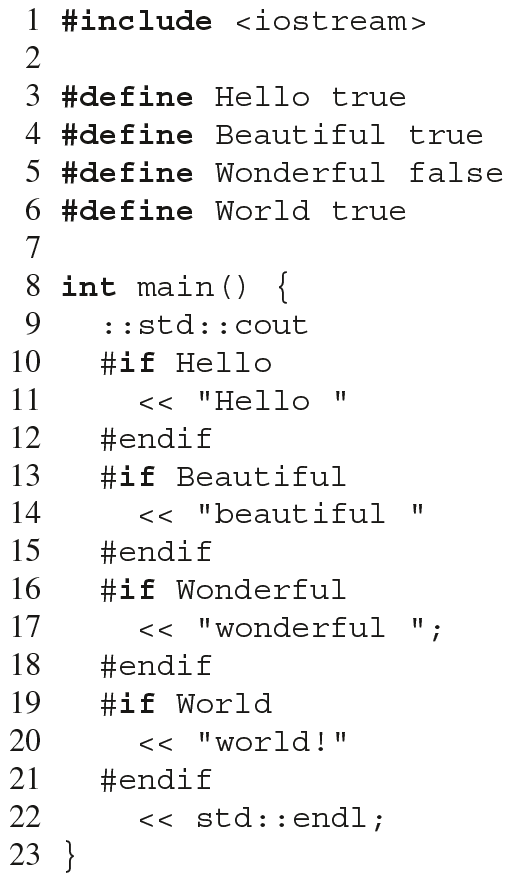
\includegraphics[scale=.3]{preprocessor-c}}
	}{
		\myexampletight{Example Output (Simplified)}{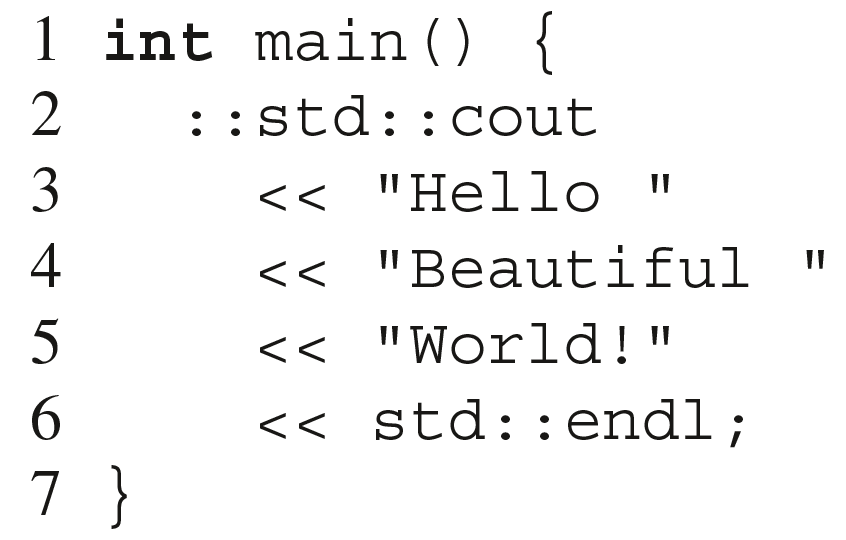
\includegraphics[scale=.15]{preprocessor-c-output}}
	}
\end{frame}
% TODO #if in above example? does this work?
% TODO keywords: #ifdef #endif #else
% TODO illustrate parameters and the call of the preprocessor

\begin{frame}{\myframetitle\ -- In a Coconutshell}
	\todots
\end{frame}
% TODO explain the most important commands: #if #defined or and not ... #elif
% TODO #include

% TODO #error
% TODO parameters, #define, even combinations

% TODO single characters
% TODO discipliced, undisciplined

\subsection{Preprocessors for Java}
\begin{frame}{Munge -- A Simple Preprocessor for Java \mytitlesource{\featureide}}
	\begin{mycolumns}[widths={55}]
		\myexampletight{Example Input and Output}{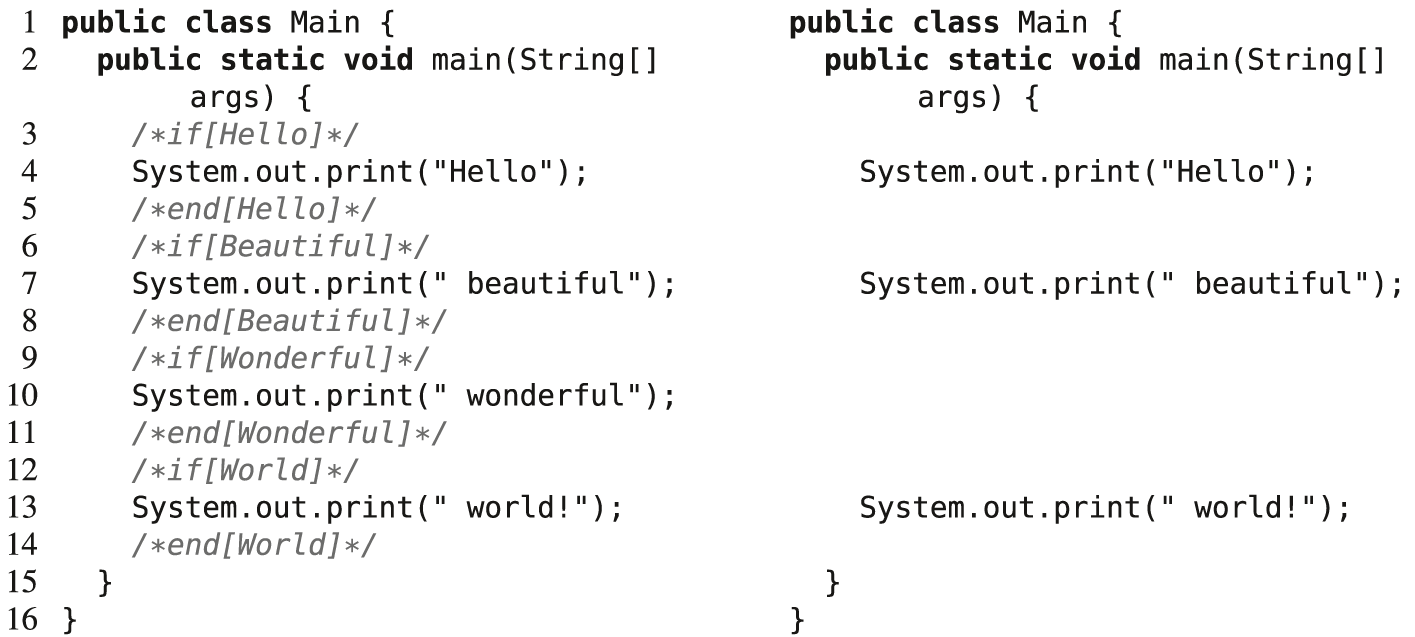
\includegraphics[width=\linewidth]{preprocessor-munge}}
	\mynextcolumn
		\myexampletight{Calling the Preprocessor}{
			\centering
			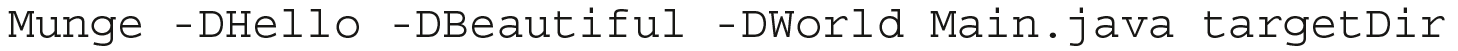
\includegraphics[width=\linewidth]{preprocessor-munge-call}
			
			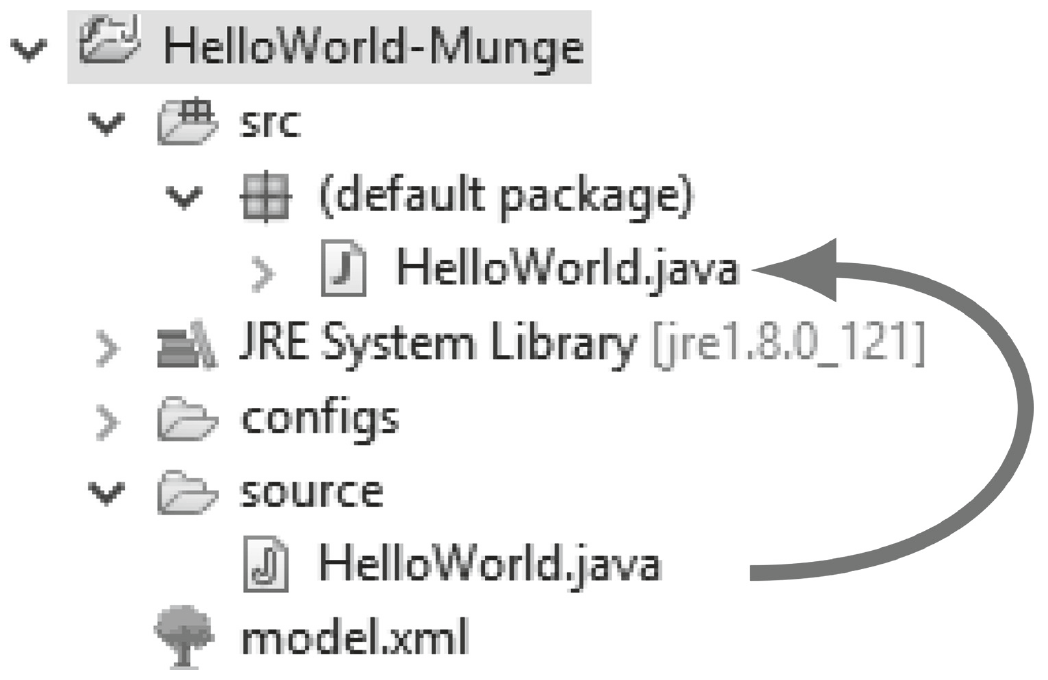
\includegraphics[width=.7\linewidth]{preprocessor-munge-idea}
		}
	\end{mycolumns}
\end{frame}

\begin{frame}{Antenna -- An In-Place Preprocessor for Java \mytitlesource{\featureide}}
	\begin{mycolumns}[widths={55}]
		\myexampletight{Example Input and Output}{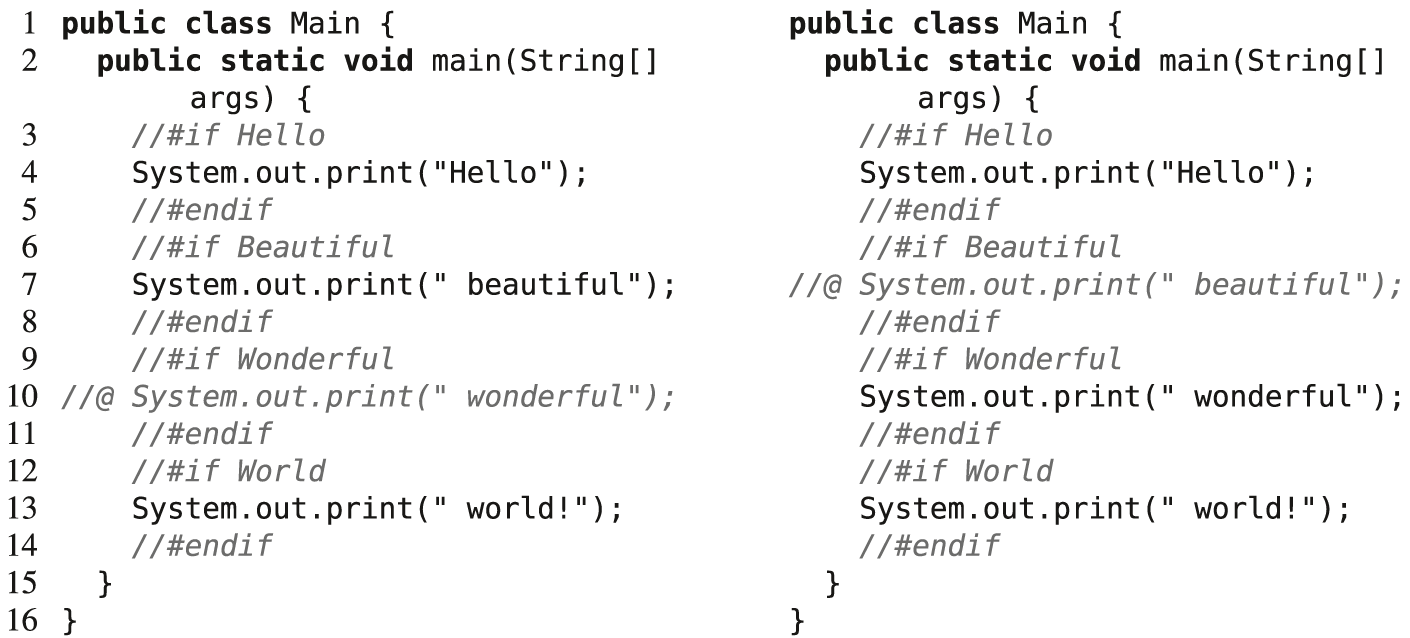
\includegraphics[width=\linewidth]{preprocessor-antenna}}
	\mynextcolumn
		\myexampletight{Calling the Preprocessor}{
			\centering
			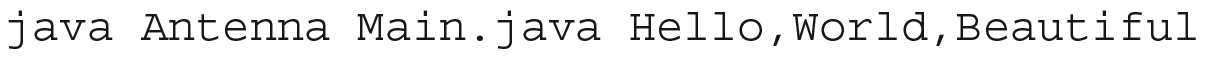
\includegraphics[width=\linewidth]{preprocessor-antenna-call}
			
			~
			
			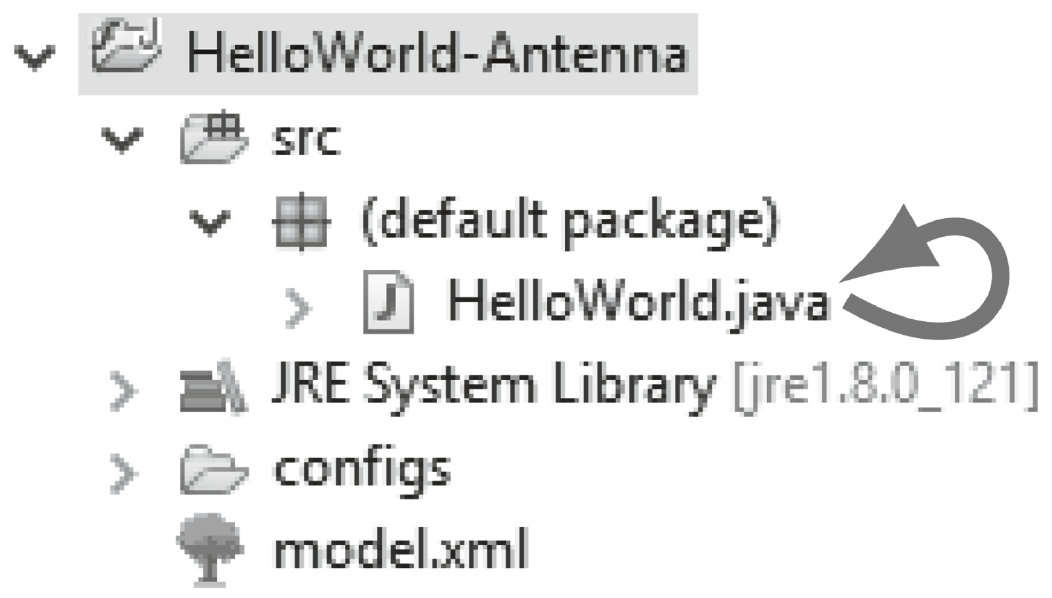
\includegraphics[width=.7\linewidth]{preprocessor-antenna-idea}
		}
	\end{mycolumns}
\end{frame}

\subsection{Preprocessors in FeatureIDE}
\begin{frame}{\myframetitle}
	\todots
\end{frame}
% has FeatureIDE been shown/discussed before? ideally, here only present preprocessor integration
% \href{https://www.youtube.com/watch?v=jVe7f32mLCQ}{demo video available} (first 2 minutes): preprocessing with Antenna on command line, feature modeling, warnings for unreferenced features, content assist proposing feature names, configuration, automated regeneration

\subsection{Discussion of Preprocessors}
\begin{frame}{\myframetitle\ \mytitlesource{\featureide}}
	\leftorright{
		\myexampletight{A Slightly More Complex Example}{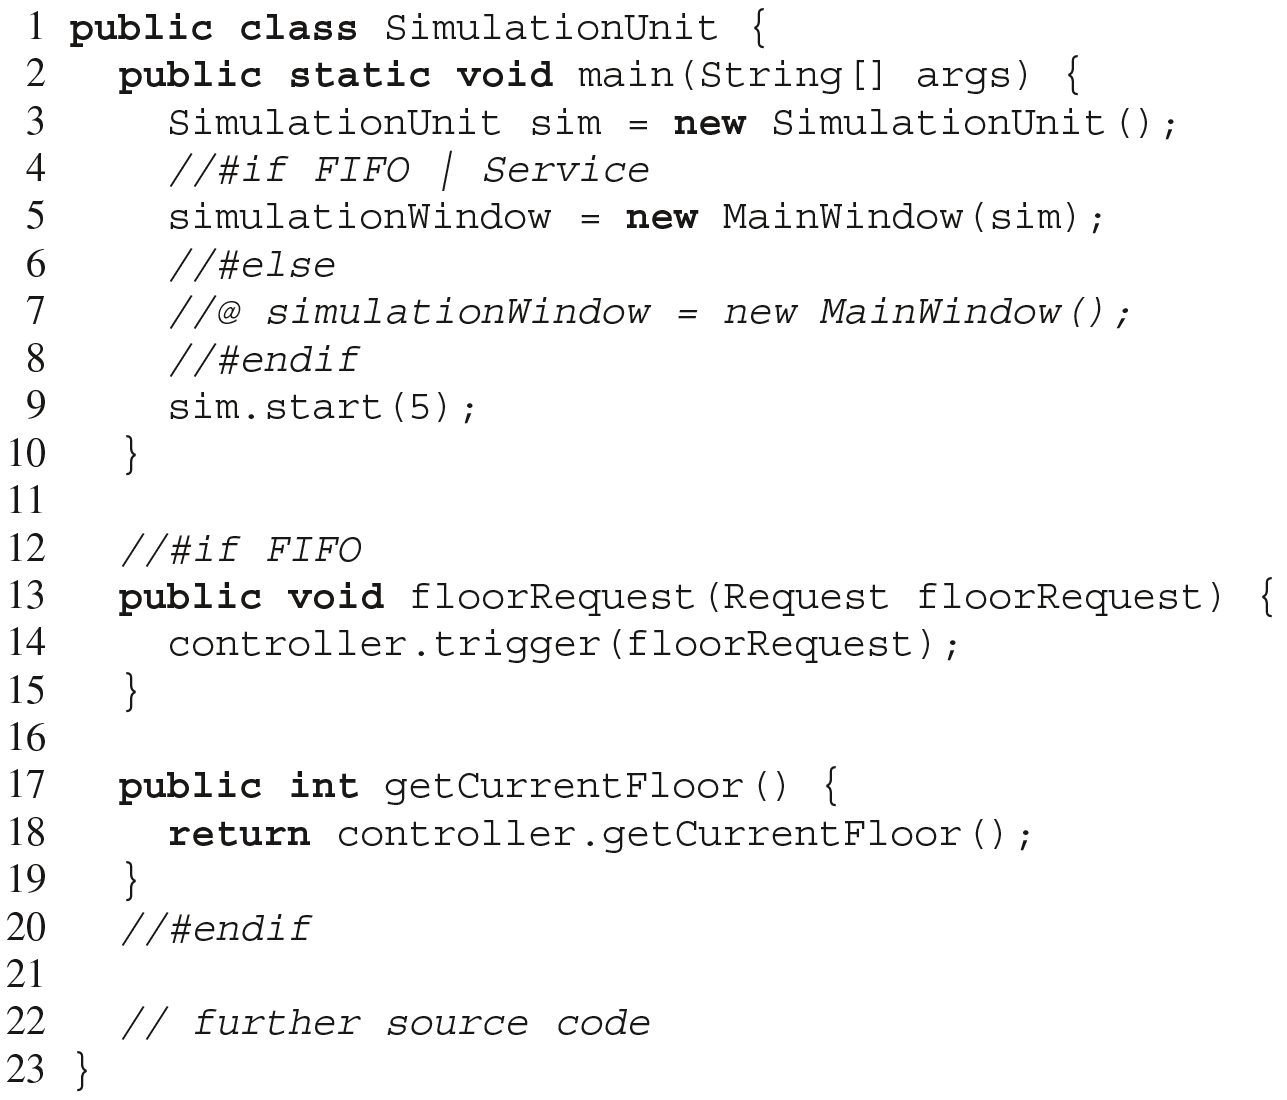
\includegraphics[width=\linewidth]{preprocessor-antenna-elevator}}
	}{
		\todots
	}
\end{frame}
% pros: fine granular, language-independent
% cons: IDE support, easy to create mistakes

\xkcdframe{619} % linux features 20s

\subsection{Preprocessor-Based Product Lines in the Wild}
\begin{frame}{\myframetitle}
	\leftorright{
		\myexample{\mysource{Liebig ICSE10}}{
			\todo{lines of code vs number of features}
		}
	}{
		\myexample{\mysource{Liebig ICSE10}}{
			\todo{number of features vs lines of variable code}
		}
	}
	\todo{add logos of all 40 systems}
\end{frame}
% TODO add pictures from Rodrigues et al. @ INFSOF’16 (Assessing fine-grained feature dependencies): methods with directives vs product lines



\lessonslearned{
	\item \ldots
}{
	\item \ldots
}{
	\ldots
}

\sectionend

\section{Feature Traceability}

\subsection{The Feature Traceability Problem}
\begin{frame}{\myframetitle}
	\begin{mycolumns}
		\todots
	\mynextcolumn
		\todots
	\end{mycolumns}
\end{frame}

\subsection{Feature Location}
\begin{frame}{\myframetitle}
	\begin{mycolumns}
		\todots
	\mynextcolumn
		\todots
	\end{mycolumns}
\end{frame}

\subsection{Feature Traceability with Colors}

\subsubsection*{FeatureCommander}
\begin{frame}{\myframetitle}
	\centering\pic[height=\textheightwithtitle]{feature-commander1}
\end{frame}
\begin{frame}{\myframetitle}
	\centering\pic[height=\textheightwithtitle]{feature-commander2}
\end{frame}
% TODO keywords on feature commander + references

\subsubsection*{FeatureIDE}
\begin{frame}{\myframetitle}
	\begin{mycolumns}
		\myexampletight{Tool Support for Feature Traceability}{\pic[width=\linewidth]{feature-traceability}}
	\mynextcolumn
		\todots
	\end{mycolumns}
\end{frame}

\subsection{Recap: Scattering, Tangling, Replication}
\begin{frame}{\myframetitle}
	\begin{mycolumns}
		\todots
	\mynextcolumn
		\todots
	\end{mycolumns}
\end{frame}

\subsection{Virtual Separation of Concerns}
\begin{frame}{\myframetitle}
	\begin{mycolumns}
		\todots
	\mynextcolumn
		\todots
	\end{mycolumns}
\end{frame}

\subsubsection*{CIDE}
\begin{frame}{\myframetitle}
	\begin{mycolumns}[widths={70},animation=none]
		\pic[width=\linewidth,trim=0 10 0 0,clip]{cide-open-editor}
	\mynextcolumn
		\begin{example}{What is CIDE?}
			\begin{itemize}
				\item stands for Colored IDE
				\item based on Eclipse and FeatureIDE
				\item special editors available for several languages:
			\end{itemize}
			\begin{flushleft}
				ANTLR, C (experimental), C++ (experimental), C\#, ECMAScript (JavaScript), Featherweight Java, \textbf{Java 1.5}, gCIDE, Haskell, JavaCC, and Python
			\end{flushleft}
		\end{example}
	\end{mycolumns}
\end{frame}

\begin{frame}{\myframetitle}
	\begin{mycolumns}[widths={70},animation=none]
		\pic[width=\linewidth]{cide-editor-and-outline}
	\mynextcolumn
		\begin{example}{Why colors?}
			\begin{itemize}
				\item colors replace preprocessor directives
				\item annotation based on syntax of the language
				\item easy annotation with selection and context menu
				\item no need to handle separators and logical connectors:\\\mycite{\texttt{,}}, \mycite{\texttt{||}}
			\end{itemize}
		\end{example}
	\end{mycolumns}
\end{frame}

\begin{frame}{\myframetitle}
	\begin{mycolumns}[widths={70},animation=none]
		\pic[width=\linewidth]{cide}
	\mynextcolumn
		\begin{example}{Why virtual separation?}
			\begin{itemize}
				\item source code is a view on the abstract syntax tree (AST)
				\item possible to hide irrelevant features
				\item possible to show overlapping features
				\item supporting development despite scattering and tangling
			\end{itemize}
		\end{example}
	\end{mycolumns}
\end{frame}

\begin{frame}{\myframetitle}
	\pic[width=\linewidth]{cide-show-single-feature}
	\begin{example}{}\centering
		possible to only show a single feature -- in its surrounded code
	\end{example}
\end{frame}

\begin{frame}{\myframetitle}
	\begin{mycolumns}[widths={45},animation=none]
		\begin{example}{Why configuration?}
			\begin{itemize}
				\item features specified in FeatureIDE feature model
				\item configuration created in FeatureIDE configuration editor
				\item configuration used to generate and visualize variant
				\item \ldots
			\end{itemize}
		\end{example}
	\mynextcolumn
		\pic[width=\linewidth]{cide-feature-selection}
	\end{mycolumns}
\end{frame}

\begin{frame}{\myframetitle}
	\begin{mycolumns}[widths={45},animation=none]
		\begin{example}{Why configuration?}
			\begin{itemize}
				\item \ldots
				\item variant visualized in source code and project explorer
				\item only necessary to press CIDE button in project explorer
				\item pressing it again returns to the view of the product line
			\end{itemize}
		\end{example}
	\mynextcolumn
		\pic[width=\linewidth]{cide-variant-view-in-project-explorer}
	\end{mycolumns}
\end{frame}
% CIDE literature
% forward reference to physical separation of concerns in next two lectures


\lessonslearned{
	\item \ldots
}{
	\item \ldots
}{
	\ldots
}

\mode<beamer>{
	\begin{frame}{\inserttitle}
		\lectureseriesoverview
	\end{frame}

	\contentoverview
}


\end{document}
